\documentclass{beamer}
\usepackage{graphicx,amsmath,amsfonts,amssymb,listings,tikz}
\usepackage{multimedia}
\usetheme{Montpellier}
\usecolortheme{beaver}
\beamerdefaultoverlayspecification{<+->}

\begin{document}

\section{Group Meeting}
\title{Group Meeting \\ Week 6, Spring 2019}
\author{Brandon Gusto} %
\institute{Dept. of Scientific Computing \\ Florida State University}
\date{\today}
\frame{\titlepage}

\begin{frame}{Multiresolution Flux Scheme}
  Currently the following operations are being performed
  \begin{enumerate}
    \item<2-> forward wavelet transform on density data
    \item<3-> construction of a mask
    \item<4-> conversion of density flux to a cell-average interpretation
      \[ R_{i}^{L} = F_{i+1/2}^{L} - F_{i-1/2}^{L} \]
    \item<5-> replacing certain cells with interpolation, based on mask information
      \[ R_{2i+1}^{l+1} = \sum_{l} \gamma_{l} R_{i}^{l} \]
      \[ R_{2i}^{l+1} = 2 R_{i}^{l} - R_{2i+1}^{l} \]
  \end{enumerate}
\end{frame}


\begin{frame}{Preliminary Results}
  The following movies show active cells in the hierarchy (top) and detail coefficients of the
  density transform (black) and density flux transform(red) (bottom). This is
  Two Blast Waves problem.
  \begin{figure}
    \center
    \movie[width=0.5\textwidth,height=0.4\textwidth, poster]{}{detailcoeff_lores.avi}
  \end{figure}
\end{frame}

\begin{frame}{Preliminary Results}
    Same data here but with a smaller tolerance.
  \begin{figure}
    \center
    \movie[width=0.5\textwidth,height=0.4\textwidth, poster]{}{detailcoeff_hires.avi}
  \end{figure}
\end{frame}

\begin{frame}{Preliminary Results}
    Here is a plot of the density over time for the same problem (low
    resolution).
  \begin{figure}
    \center
    \movie[width=0.5\textwidth,height=0.4\textwidth, poster]{}{density_lores.avi}
  \end{figure}
\end{frame}

\begin{frame}{Preliminary Results}
    Density over time for higher resolution.
  \begin{figure}
    \center
    \movie[width=0.5\textwidth,height=0.4\textwidth, poster]{}{density_hires.avi}
  \end{figure}
\end{frame}

\begin{frame}{Preliminary Results}
  Proportion of active cells at the finest level during the simulation.
  \begin{figure}
    \center
    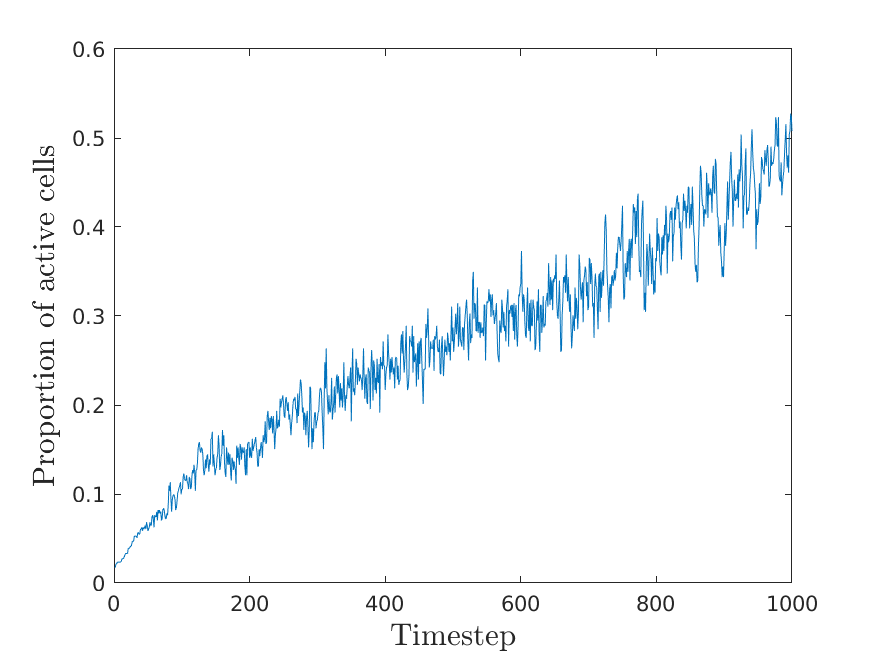
\includegraphics[scale=0.5]{numactive_lores.png}
  \end{figure}
\end{frame}

\begin{frame}{Preliminary Results}
  Proportion of active cells at the finest level during the simulation (higher tolerance).
  \begin{figure}
    \center
    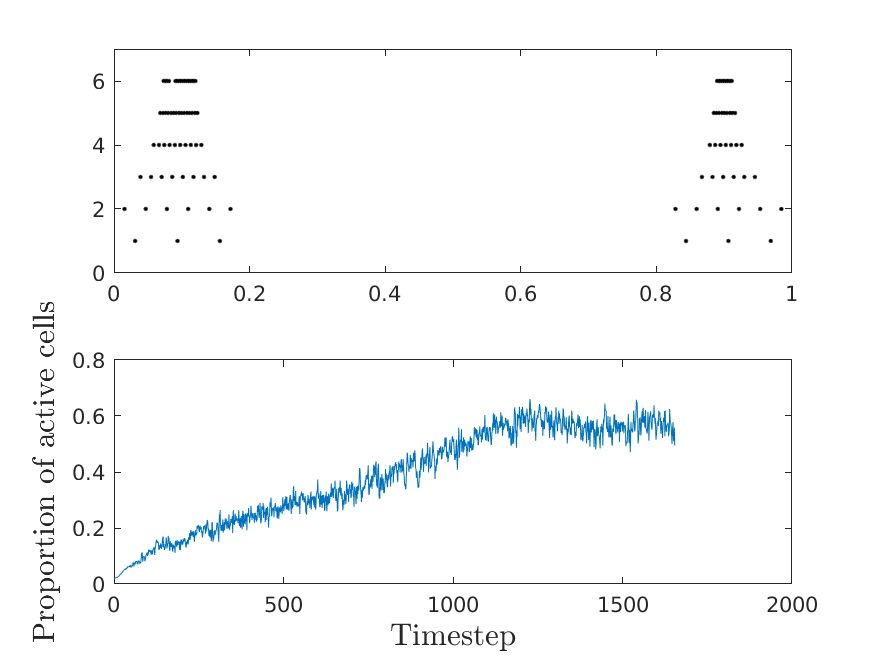
\includegraphics[scale=0.5]{numactive_hires.png}
  \end{figure}
\end{frame}

\begin{frame}[fragile]{To-Do List}
  Several items needing attention are
  \begin{itemize}
    \setlength\itemsep{1em}
    \item<2-> set wavelet threshold in \texttt{flash.par}
    \item<3-> set refinement variables there as well
  \end{itemize}
  Later on will need to...
  \begin{itemize}
    \item<4-> test a suite of problems
    \item<5-> run on parallel blocks
    \item<6-> compare solutions obtained via MR with non-MR
    \item<7-> pass a non-uniform array to \texttt{hydro\_1d.F90}, test efficiency
  \end{itemize}
\end{frame}

\end{document}
